%%%% Ecriture du plan

\section*{Introduction}

\section{Etat de l'art}

\subsection{Problématiques et historique}

\begin{figure}[h!]
  \centerline{
  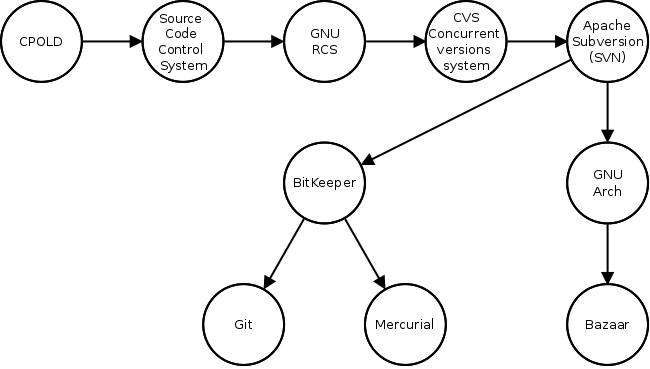
\includegraphics[width=14cm]{images/chronologie.png}}
  \caption{Résumé des gestionnaires de versions à travers l'histoire}
  \label{fig:chronologie}
\end{figure}

\subsection{Cahier des charges d'un gestionnaire de versions}

On récapitule toutes les fonctionnalités clés : branches, commit, merge, stage, repo, centralisé, décentralisé, diff

\subsection{Récapitulatif/Comparatif des gestionnaires de versions}

- bitkeeper, git
 - cvs, svn

\section{Etude de GIT}

\subsection{Choix de GIT}

\subsection{Utilisation de GIT}

\subsection{Détails sur le fonctionnement de GIT}

\section*{Conclusion}


